\scanpage{176}
infinité de termes].

Soit $\varphi_*$ un \uline{\unsure{endomorphisme}} de la
$k$-algèbre diff. $\unsure{\tfrac12}$-simpliciale $\mathcal A_{k*}^\wedge$, associé à
\[
 A,\unsure{B}_i\in\widehat S_k\{\{X_0\}\}\simeq
 k\{\{T\}\}\{\{X_0\}\}\simeq k\{\{X_0,X_1\}\}
 \qquad(i\geq1)
\]
Posons
\[
 \left\{\begin{aligned}
 A&=\sum_{j\geq1}a_jX_0^{(j)}
 &&(a_j\in\widehat S_k\simeq k\{\{T\}\},j>0)\\
 \text{avec }a_j&=\sum_{h\geq0}a_{j,h}T^{(h)},
 &&a_{jh}\in k\quad\text{pour }j\geq1,h\geq0
 \end{aligned}\right.
\]
On peut aussi écrire
\[
 \left\{A=\sum_{\substack{i\geq1\\j\geq0}}\alpha_{ij}X_0^{(i)}X_1^{(j)}
 \qquad\alpha_{ij}\in k\right.
\]
Posons
\[
 \varphi_0(T)=\sum_{j\geq1}\lambda_jT^{(j)}\qquad\lambda_j\in k
\]
Ceci posé un calcul immédiat montre
\[
 \boxed{a_{1,0}=\alpha_{1,0}=\lambda_1}\quad\in k.
\]
Cet élément de $k$ s'appelle le
\deleted{\uline{indicateur}}\inserted{\deleted{discriminant}\inserted{déterminant}}
de $\varphi_*$, \inserted{noté $\Delta(\varphi_*)$}
(on peut aussi en définir si on a
$\varphi_*:\mathcal A_k^\wedge\longrightarrow \mathcal A_{k'}^\wedge$ associé à
$k\mathbin{\text{---}}k'$ donné d'avance, on trouve un élément de $k'$).

\uline{Théorème} Pour que $\varphi_*$ soit un \uline{autom.}
de $\mathcal A_{k*}^\wedge$, il f. et s. que son indicateur
soit un élément inversible de $k$. En tous cas, $\Delta(\varphi_*)$ dépend multiplicativement
de $\varphi_*$, et $\Delta(\mathrm{Id})=1$ -- donc $\Delta$ est un hom de gr.
\[
 \Omega(k)=\operatorname{Aut}_{k\,\mathrm{alg}\,\mathrm{diff}\,\unsure{\frac12\mathrm{simp}}}(\mathcal A_{k*}^\wedge)
\]
dans $k^*=G_m(k)$.
\figure{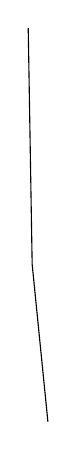
\begin{tikzpicture}\draw (0,5)--(.05,2)--(.25,0);\end{tikzpicture}}
\margin{175}
